% =============================================================================================
% STANDALONE EXPORT OF §6 AND APPENDICES D–E FOR EXTERNAL COLD REVIEW.
%
% Exported verbatim from the manuscript; nothing is re-typed, so the export cannot drift. §6's
% three figure floats live in sections/06_figures.tex, shared with main.tex.
%
% Appendices A–C are NOT here — they shipped with the §3 export (review_s3.pdf) because they are
% load-bearing for §3's argument. D and E are new and stand alone.
%
% Build:  tectonic -X compile paper/review_s6.tex
% =============================================================================================
\documentclass[10pt]{article}
\usepackage{preprint}

\author{}
\date{}

\begin{document}

% Bind every out-of-export label to the number it carries in the manuscript, so each reference
% resolves to what a reader of the full paper would see.
\makeatletter
\@namedef{r@sec:mechanism}{{3}{1}{Capacity eviction}{section.3}{}}
\@namedef{r@sec:mechanism@cref}{{[section][3][]3}{1}}
\@namedef{r@sec:mech-predict}{{3.3}{1}{The prediction, tested}{subsection.3.3}{}}
\@namedef{r@sec:mech-predict@cref}{{[subsection][3][3]3.3}{1}}
\@namedef{r@sec:mech-gate}{{3.7}{1}{Verification and the gate}{subsection.3.7}{}}
\@namedef{r@sec:mech-gate@cref}{{[subsection][7][3]3.7}{1}}
\@namedef{r@sec:decision}{{4.6}{1}{The decision rule}{subsection.4.6}{}}
\@namedef{r@sec:decision@cref}{{[subsection][6][4]4.6}{1}}
\@namedef{r@sec:lim-baseline}{{7.2}{1}{The BSQ baseline is ours}{subsection.7.2}{}}
\@namedef{r@sec:lim-baseline@cref}{{[subsection][2][7]7.2}{1}}
\@namedef{r@sec:lim-placebo}{{7.3}{1}{The placebo removes information and capacity together}{subsection.7.3}{}}
\@namedef{r@sec:lim-placebo@cref}{{[subsection][3][7]7.3}{1}}
\@namedef{r@sec:lim-power}{{7.4}{1}{The effect we can detect is larger than the effect we expect}{subsection.7.4}{}}
\@namedef{r@sec:lim-power@cref}{{[subsection][4][7]7.4}{1}}
\@namedef{r@sec:lim-matching}{{7.8}{1}{Two matching caveats}{subsection.7.8}{}}
\@namedef{r@sec:lim-matching@cref}{{[subsection][8][7]7.8}{1}}
\@namedef{r@sec:repro-prereg}{{8.4}{1}{Pre-registration and the amendment log}{subsection.8.4}{}}
\@namedef{r@sec:repro-prereg@cref}{{[subsection][4][8]8.4}{1}}
\makeatother

\setcounter{section}{5}   % so §6 numbers as §6
\setcounter{figure}{7}    % Figures 1--7 precede this section
\setcounter{table}{0}

{\centering
{\normalsize\textsc{Section 6 and Appendices D--E --- export for external review}}\\[0.5em]
{\Large\bfseries Capacity Eviction in Reconstruction-Trained Tokenizers}\\[0.4em]
{\small\color{tolgrey} Draft of \today\ --- text frozen pending review}\\[1.6em]
}

\noindent\textbf{Note to the reviewer.} \S6 reports the outcome of a pre-registered experiment
that \textbf{has not been executed}. Every quantity in it is an empty slot, marked in red, bound
to a named field of the verdict manifest; the three figures are drawn on placeholder data that is
implausible by construction. Nothing in \S6 is a measurement, and the section is written so that
a paragraph or panel cropped out of context cannot be mistaken for one. Appendices D and E are
complete and contain no pending values except where explicitly marked. Appendices A--C are not
reproduced here --- they shipped with the \S3 export.

\medskip
\noindent\textbf{Why this is worth reviewing before the run.} The purpose of pre-writing \S6 is
that the distance from ``verdict lands'' to ``submittable'' should be a mechanical substitution
rather than a writing task, and that neither interpretation can be composed with an outcome in
front of us. \S6.5 therefore contains \emph{both} interpretation paragraphs, written and dated
2026-08-10. Exactly one will be retained; the other will be deleted rather than softened.

\medskip
\noindent\textbf{What we would most like challenged.}
(i) Whether the \textsc{survives} paragraph in \S6.5 concedes enough --- it claims an existence
proof on one slice and binds itself with three limits, and we would like to know whether a
referee reads it as appropriately narrow or as hedged into meaninglessness.
(ii) Whether the \textsc{null} paragraph is honest or self-serving: it argues a pre-registered
null is a contribution to the record, and that is exactly the argument an author with a null
would want to make.
(iii) Whether any slot in \S6 could be filled in more than one defensible way --- the intent is
that each binds to exactly one manifest field, so if a reviewer can see a judgement call, the
binding is under-specified.
(iv) Whether the placeholder figures are genuinely impossible to mistake for results with the
watermark removed.
(v) In Appendix E, whether the four-status scheme (measured / derived / \emph{pin} / pending) is
the right cut, and whether anything currently labelled a pin is being used as evidence anywhere
in the paper.
(vi) Anything in Appendix D that a reader would need in order to check a run against the
pre-registration and cannot find there.

\bigskip
\hrule
\bigskip

% =============================================================================================
% §6 Results — STRUCTURED STUBS ONLY. The pre-registered run has not been executed.
%
% CONTEXT-STRIPPING RULE (CLAUDE.md standing rules). Every slot below is \TBD{} or \PH{}, in red,
% and NO slot contains a plausible value. A reader who crops a paragraph out of this section must
% not be able to mistake any of it for a measurement. When the run lands, each \TBD is replaced
% from a single named field of the verdict manifest -- the field is named beside every slot so the
% substitution is mechanical and cannot be improvised.
%
% BOTH interpretation paragraphs in §6.6 are written NOW and dated, before any result exists, so
% that neither can be tuned to an outcome. That is the point of writing them here.
% =============================================================================================
\section{Results}
\label{sec:results}

\emph{The pre-registered run has not been executed. Every quantity in this section is an empty
slot bound to a named field of the verdict manifest, and every figure is drawn on placeholder data
that is implausible by construction. Nothing here is a measurement.}

\subsection{The pre-second-stage gate}
\label{sec:res-gate}

The legibility gate of \cref{sec:mech-gate} runs on real data before any second-stage training is
authorized, and it is a hard stop rather than a diagnostic: it requires at least $0.90$ sign
accuracy on \emph{every one} of the six live microstructure dimensions, with no mean clause and no
floor. Its outcome determines whether the rest of this section exists.

\begin{center}
\begin{tabular}{ll}
\toprule
quantity & value \\
\midrule
per-dimension sign accuracy, dims 7--12 & \TBD{six values} \\
minimum across the six & \TBD{min} \\
gate outcome & \TBD{pass or hard stop} \\
\bottomrule
\end{tabular}
\end{center}
% manifest binding: gates.gate2_legibility.{new_by_seed, min, threshold=0.90, pass}

\subsection{Primary outcome}
\label{sec:res-primary}

The five clauses of \cref{sec:decision} are evaluated conjunctively: the primary outcome is
\textsc{survives} only if none fails, and \textsc{null} otherwise. Two guards sit outside the
clauses and are \textsc{halt}-only. \Cref{fig:verdict} draws the surface.

\begin{center}
\begin{tabular}{lll}
\toprule
clause & tests & outcome \\
\midrule
1 paired CI & $\Delta\IR(4-5)$ lower bound $> 0$ & \TBD{} \\
2 MDE & $\Delta\IR(4-5) \ge$ paired MDE & \TBD{} \\
3 placebo validity & $\IR(4) - \IR(2)$ lower bound $> 0$ & \TBD{} \\
4 economic floor & materiality against the $0.5$ floor & \TBD{} \\
5 deflated Sharpe & against $SR_0$ at $N = 60$ trials & \TBD{} \\
\midrule
degeneracy guard & constant-direction book, any cell & \TBD{halt or clear} \\
power guard & across-seed range vs claimed effect & \TBD{halt or clear} \\
\midrule
\textbf{primary} & & \TBD{SURVIVES / NULL / INCONCLUSIVE} \\
\bottomrule
\end{tabular}
\end{center}
% manifest binding: clauses.{1_paired_ci, 2_mde_paired, 3_placebo_validity, 4_economic_floor,
% 5_dsr}.passed; degeneracy_guard.halted; power_guard.halted; primary. The rule STRINGS printed in
% Fig 8 are read from the manifest, not restated.

Both specifications required by the amendment window are reported from the same artifacts, and
their agreement or disagreement is stated here rather than in a footnote.

\begin{center}
\begin{tabular}{lll}
\toprule
 & v1.5 specification (primary) & retained alternative \\
\midrule
primary outcome & \TBD{} & \TBD{} \\
specifications agree & \multicolumn{2}{l}{\TBD{yes or no --- a first-class finding either way}} \\
\bottomrule
\end{tabular}
\end{center}
% manifest binding: dual_specification.* — a manifest lacking this field cannot be quoted (§7 v1.5)

\subsection{Effect sizes and secondary diagnostics}
\label{sec:res-effects}

Information coefficient, rank information coefficient, mean absolute error and $R^2$ are reported
as secondary diagnostics and do not enter the decision rule.

\begin{center}
\begin{tabular}{lccccc}
\toprule
cell & 1 BSQ/OHLCV & 2 FSQ/OHLCV & 3 BSQ/+micro & 4 FSQ/+micro & 5 placebo \\
\midrule
net IR, seed mean & \TBD{} & \TBD{} & \TBD{} & \TBD{} & \TBD{} \\
across-seed range & \TBD{} & \TBD{} & \TBD{} & \TBD{} & \TBD{} \\
RankIC & \TBD{} & \TBD{} & \TBD{} & \TBD{} & \TBD{} \\
decision activity at $\kappa^\ast$ & \TBD{} & \TBD{} & \TBD{} & \TBD{} & \TBD{} \\
\bottomrule
\end{tabular}
\end{center}
% manifest binding: per_cell.{ir_seed_mean, ir_range_across_seeds, rankic}; degeneracy_guard.
% per_cell.activity_decisions_seed_mean. The activity row is printed whatever it reads, per §4.4.

The three marginals involving a BSQ arm are reported and not claimed, for the reason
\cref{sec:lim-baseline} gives, and the required disclosure ships with them verbatim.

\subsection{Cost stress and seed dispersion}
\label{sec:res-stress}

\Cref{fig:cost} sweeps the round-trip cost around the pinned $0.30\%$; \cref{fig:seeds} plots each
cell's five seeds against the size of the effect being claimed. Both figures are built against the
manifest schema and are watermarked until the run lands.

\subsection{Interpretation}
\label{sec:res-interpretation}

\emph{Both paragraphs below were written on 2026-08-10, before the run was executed and before any
result existed. Exactly one will be retained; the other is deleted rather than softened. They are
placed here, in advance, so that neither can be written to fit an outcome.}

\paragraph{If the outcome is \textsc{survives}.} A positive $\Delta\IR(4-5)$ that clears the
paired confidence interval, the minimum detectable effect, the economic floor and the deflation
benchmark establishes that real trade-flow imbalance carries information beyond input capacity, and
that a tokenizer built to preserve it delivers that information to a cost-aware trading decision.
The claim ends there, and three limits bind it immediately. It is not a calibrated estimate of how
much: \cref{sec:lim-placebo} states that $\Delta\IR(4-5)$ mixes information with an unquantified
capacity handicap, so the measured difference is an upper bound on the information effect rather
than an estimate of it. It is not evidence that our BSQ baseline is competitive, so the
quantizer-axis marginals remain reported rather than claimed. And it is one exchange, one venue,
one instrument class and one year of scored data, with no regime-transfer test --- a positive
result here is an existence proof on this slice, not a property of markets. The mechanism of
\cref{sec:mechanism} would remain a fixture result; a positive outcome is consistent with it and
does not confirm it, because many differences between cells 2 and 4 could produce the same sign.

\paragraph{If the outcome is \textsc{null} or \textsc{inconclusive}.} This is the outcome the
design's own arithmetic makes most likely, and we pre-committed it as publishable before any result
existed, so it is reported without reframing. A null here means that under this pre-registered
decision rule, at this budget, on this slice, the microstructure arm did not beat its placebo by a
margin the design could resolve. It does \emph{not} mean microstructure carries no information: the
minimum detectable effect is $3.518$ annualized IR against a prior of $|\text{RankIC}| = 0.027$, so
the design would fail to detect a real effect of the size we actually expect, and
\cref{sec:lim-power} states that the effect we can detect is larger than the effect we predict.
Nor does it mean the mechanism of \cref{sec:mechanism} is wrong --- the mechanism is established on
a fixture and is not contingent on this outcome. What a null does establish is narrower and still
worth publishing: that the pipeline, with the interface defect removed and the legibility gate
passed, does not convert this microstructure signal into net information ratio at this scale.
Given how much of this literature reports only positive results, a pre-registered null with its
power analysis stated in advance is a contribution to the record rather than a failed experiment.
\Cref{sec:lim-power} names what would change the answer: more scored data, a lower-cost venue, or
an effect larger than our own prior.

% The three figures belonging to §6. Held in their own file so main.tex and review_s6.tex
% share one copy and the export cannot drift from the manuscript.
\begin{figure}[t]
  \centering
  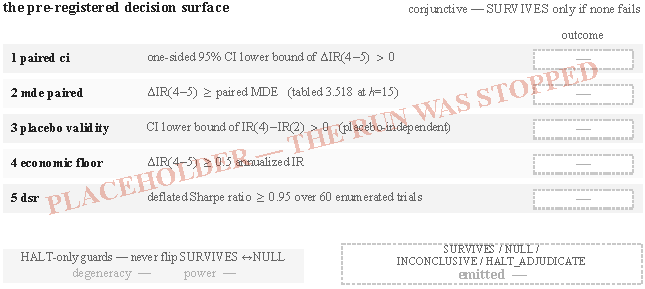
\includegraphics[width=\textwidth]{figures/fig8_verdict.pdf}
  \caption{\textbf{The decision surface, fixed before any result existed.} Five clauses, evaluated
  conjunctively: the primary outcome is SURVIVES only if none fails, and NULL otherwise. Two
  guards sit outside the clauses and are HALT-only --- they can refuse to report an outcome their
  own inputs cannot support, and can never flip SURVIVES to NULL or back. The rule strings shown
  are transcribed into this figure's source rather than loaded from a manifest, and are therefore a
  restatement; the persisted strings are the authority. \PH{no values} --- every outcome
  cell is empty because the run has not been executed; each is filled from a single named field of
  that manifest.}
  \label{fig:verdict}
\end{figure}
\clearpage
\begin{figure}[t]
  \centering
  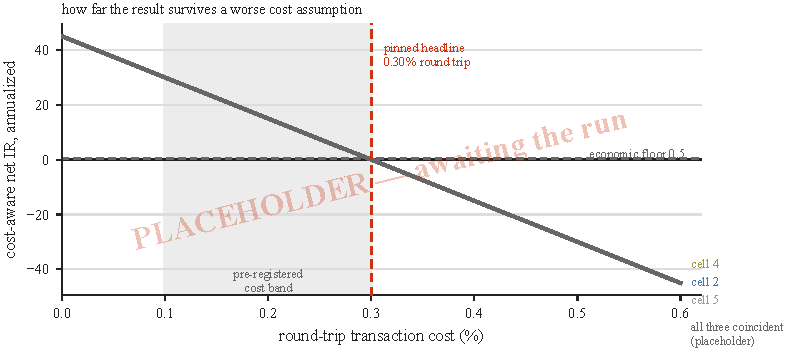
\includegraphics[width=\textwidth]{figures/fig9_cost_stress.pdf}
  \caption{\textbf{The specified cost-stress apparatus, with no curve.} Cost-aware net information
  ratio against the round-trip transaction cost was to be drawn here for the microstructure arm,
  the OHLCV-only arm and the placebo; the headline is pinned at $0.30\%$, the pessimistic end of
  the pre-registered $0.1$--$0.3\%$ band. \PH{no curve drawn} --- the ablation this panel was
  specified for never ran, so the axes, the pinned rate, the band and the economic floor are real
  and no cell is drawn. An earlier draft carried a placeholder line whose zero crossing fell
  \emph{exactly} on the pinned $0.30\%$ rule, the most quotable point on the axis; cropped away
  from this caption it read as a break-even of $0.30\%$, against a measured $0.0023$--$0.0208\%$.
  The one break-even we have measured is drawn instead, in red at the left margin, with its
  cell-1-only scope written into the image rather than left to the caption.}
  \label{fig:cost}
\end{figure}
\clearpage
\begin{figure}[t]
  \centering
  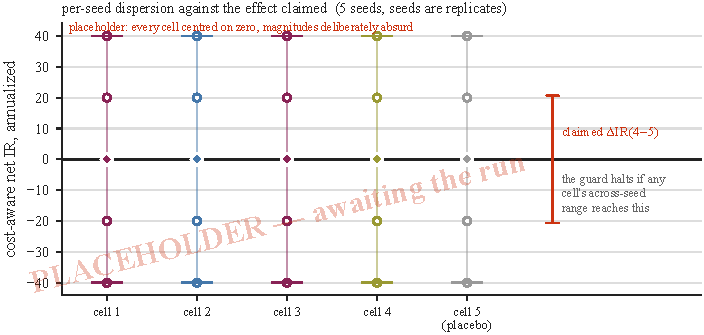
\includegraphics[width=\textwidth]{figures/fig10_seed_stability.pdf}
  \caption{\textbf{Seed dispersion against the effect being claimed.} Each cell's five seeds are
  replicates of one configuration, not five configurations; open circles are seeds, the diamond is
  the seed mean, and the bars mark the across-seed range. The comparison that matters is the one
  drawn on the right: if any cell's across-seed range reaches the size of the effect being claimed,
  the power guard halts and the verdict is reported as adjudication-required rather than as an
  outcome.
  \PH{every cell centred on zero, magnitudes $\sim\pm40$} --- no cell is favoured and the claimed
  effect is drawn symmetric about zero, so the panel shows the comparison's geometry and no
  result.}
  \label{fig:seeds}
\end{figure}
\clearpage



\clearpage
\appendix
\setcounter{section}{3}   % so the next \section numbers as D
% =============================================================================================
% Appendix D — the pinned decision surface, verbatim.
%
% §8 DESCRIBES the conformance surface; this appendix TABULATES it, so a reader can check a run's
% configuration against the pre-registration without reading our code. Every value below is
% imported live from src/trikaal/eval/conformance.py and src/trikaal/eval/verdict.py -- none is
% transcribed. Renamed from "Reproducibility and verification" so it does not duplicate §8's title.
% =============================================================================================
\section{The pinned decision surface}
\label{app:repro}

Every quantity below was fixed before any of its inputs existed and is hard-asserted before any
cell is scored. A run whose configuration differs from any of these raises rather than producing a
downgraded result. The values are reproduced from the constants themselves, not from prose.

\subsection*{D.1\quad Experiment pins}

\begin{center}
\begin{tabular}{lll}
\toprule
constant & value & governs \\
\midrule
\texttt{PINNED\_SYMBOLS\_SHA256} & \texttt{60e24f59\ldots dc32631} & the evaluation universe \\
\texttt{PINNED\_SEEDS} & $(0,1,2,3,4)$ & five replicates, fixed up front \\
\texttt{PINNED\_KAPPAS} & $(1.0, 1.5, 2.0, 3.0)$ & the execution-filter grid \\
\texttt{PINNED\_HEADLINE\_COST} & $0.0030$ & flat round trip, the pessimistic band end \\
\texttt{PINNED\_MONEY\_SEQ\_LEN} & $512$ & eval surface and training context \\
\texttt{PINNED\_BACKBONE\_PARAMS} & $21{,}301{,}248$ & the realized parameter count \\
\texttt{PINNED\_STEPS\_STAGE1} & $26{,}003$ & tokenizer budget, matched across arms \\
\texttt{PINNED\_STEPS\_STAGE2} & $26{,}003$ & backbone budget, matched across arms \\
\texttt{PINNED\_MU\_ESTIMATOR} & \texttt{expectation} & conditional mean, not mode \\
\texttt{PINNED\_ENCODER\_CAUSAL} & \texttt{True} & forced for every cell \\
\texttt{PINNED\_FINE\_POINTWISE} & \texttt{True} & the re-specified interface \\
\texttt{PINNED\_MICRO\_POINT\_WEIGHT} & $3.0$ & the class weight $\lambda$ \\
\texttt{PINNED\_MICRO\_LEGIBILITY\_MIN} & $0.90$ & the gate, on every live micro dimension \\
\texttt{PINNED\_CODEBOOK\_MIN\_UTILIZATION} & $0.95$ & BSQ collapse check \\
\bottomrule
\end{tabular}
\end{center}

\subsection*{D.2\quad Decision thresholds and the deflation recipe}

\begin{center}
\begin{tabular}{lll}
\toprule
constant & value & governs \\
\midrule
\texttt{ECON\_FLOOR\_IR} & $0.5$ & clause 4 materiality floor \\
\texttt{DSR\_N\_TRIALS} & $60$ & clause 5 trial count \\
\texttt{DSR\_THRESHOLD} & $0.95$ & clause 5 deflated-Sharpe threshold \\
trial factorization & cells $\times$ horizons $\times$ $\kappa$ & $5 \times 3 \times 4 = 60$ \\
\texttt{DSR\_HORIZONS} & $(5, 15, 60)$ & the horizon axis \\
\texttt{DSR\_VAR\_SR\_BASIS\_CELL} & $5$ & dispersion basis is the \emph{placebo} arm \\
de-annualization horizon & $15$ & the unit $SR_0$ is compared against \\
\texttt{PLACEBO\_DISPERSION\_TRIPWIRE} & $1.5\times$ & disclose if the placebo arm is over-dispersed \\
\texttt{PINNED\_BOOT} & $B = 10{,}000$, seed $20260704$, $\alpha = 0.05$ & the paired bootstrap \\
\texttt{BOOT\_POWER} & $0.80$ & the MDE's power term \\
\texttt{FRAC\_NEG\_BAND} & $[0.05, 0.95]$ & degeneracy guard, sign-balance leg \\
\bottomrule
\end{tabular}
\end{center}

Two conventions, stated so a reader is not left to infer them. \texttt{DSR\_N\_TRIALS} is a
\textbf{pin}, not a derived quantity: its value $60$ equals the product of the factorization
($5$ cells $\times$ $3$ horizons $\times$ $4$ values of $\kappa$), and conformance asserts both the
literal and the factorization, but the decision to enumerate trials that way was made by us before
the run and is not a measurement. \Cref{app:claims} classifies it accordingly. And
\texttt{FRAC\_NEG\_BAND} governs only the sign-balance leg of the degeneracy guard; the
filter-binding leg of the same guard tests the exact endpoints $0$ and $1$ with no band, so an
activity of $0.999$ passes where a fraction-negative of $0.999$ halts. That asymmetry is disclosed
rather than resolved: whether to band the activity leg is an open decision at the time of writing,
with no amendment superseding the current form, and \cref{sec:lim-filter} states what it leaves
uncovered.

Two of these carry a history that \cref{sec:repro-prereg} summarizes and the amendment log states
in full. The trial count was reduced from $180$ to $60$ when seeds were recognized as replicates
rather than configurations, and the dispersion basis was moved to the placebo arm because the
earlier all-arms basis made clause 5 anti-correlated with its own hypothesis. The first tightens
the criterion and the second loosens it; the net is indeterminate before the run, and
\cref{sec:repro-prereg} explains why we report it that way rather than as a single direction.

\subsection*{D.3\quad Evaluation geometry}

\begin{center}
\begin{tabular}{ll}
\toprule
quantity & value \\
\midrule
window & 2021-01-01 to 2025-01-01, one-minute bars \\
train/forward split & 2023-10-20, the $0.7$ point \\
forward blocks & $6$; block $0$ selects $\kappa$ and is excluded \\
headline region & blocks 1--5, $\approx$ 2024-01-01 to 2025-01-01 \\
periods per instrument at $h=15$ & $35{,}063$ \\
scored instruments & $40$ of the $200$ in the lake \\
effective breadth & $1.5$ \\
label look-forward & $60$ bars \\
serial-correlation margin & $60$ bars \\
leading embargo & $120$ bars \\
\bottomrule
\end{tabular}
\end{center}

\subsection*{D.4\quad Content addressing and environment}

The Gate-A anchor is a fixed evaluation of a frozen checkpoint through the full harness, re-proven
twice from unpiped commands before and after any change to the evaluation instrument.

\begin{center}
\begin{tabular}{ll}
\toprule
artifact & value \\
\midrule
anchor results hash & \texttt{sha256:3f86882a63dd06c78\ldots} \\
anchor causal sweep & $420$ of $420$ checks \\
anchor dataset hash & \texttt{sha256:1d3ec4f8db6686e2\ldots} \\
anchor tokenizer hash & \texttt{sha256:ce7c8c4ae0b62c89\ldots} \\
anchor predictor hash & \texttt{sha256:6d118ede6bfcab2e\ldots} \\
universe Merkle root & \texttt{sha256:5dfd667d05b97bda\ldots} \\
lake & $7{,}024$ Parquet files, $200$ symbols, $304{,}625{,}181$ bars \\
Python & 3.11.7 \\
NumPy & 2.4.6 \\
PyTorch & 2.12.1 \\
\bottomrule
\end{tabular}
\end{center}

The environment is pinned by a lockfile and load-bearing results are re-verified under it. The
amendment log carries $41$ distinct revision tags, each with its date, its reason, and the
direction it moves the criterion, recorded before the amendment was evaluated.

\subsection*{D.5\quad Slot-to-field bindings for \S6}

Every empty slot in \cref{sec:results} binds to exactly one named field of the verdict manifest.
The binding is recorded here so that filling \S6 after the run is a mechanical substitution rather
than a judgement, and so that a reader can check any published value against the artifact without
our assistance. A slot with more than one defensible source would be a specification defect, not a
choice; none below has one.

\begin{center}
\begin{tabular}{lll}
\toprule
\S6 slot & manifest field & type \\
\midrule
per-dimension sign accuracy & \texttt{gates.gate2\_legibility.new\_by\_seed} & 6 floats \\
minimum across the six & \texttt{gates.gate2\_legibility.min} & float \\
gate outcome & \texttt{gates.gate2\_legibility.pass} & bool \\
clause 1 outcome & \texttt{clauses.1\_paired\_ci.passed} & bool \\
clause 2 outcome & \texttt{clauses.2\_mde\_paired.passed} & bool \\
clause 3 outcome & \texttt{clauses.3\_placebo\_validity.passed} & bool \\
clause 4 outcome & \texttt{clauses.4\_economic\_floor.passed} & bool \\
clause 5 outcome & \texttt{clauses.5\_dsr.passed} & bool \\
degeneracy guard & \texttt{degeneracy\_guard.halted} & bool \\
power guard & \texttt{power\_guard.halted} & bool \\
primary outcome & \texttt{primary} & enum \\
dual-specification pair & \texttt{dual\_specification.\{primary,alternative\}} & enum $\times2$ \\
specifications agree & \texttt{dual\_specification.agree} & bool \\
net IR, seed mean & \texttt{per\_cell.\{1..5\}.ir\_seed\_mean} & 5 floats \\
across-seed range & \texttt{per\_cell.\{1..5\}.ir\_range\_across\_seeds} & 5 floats \\
RankIC & \texttt{per\_cell.\{1..5\}.rankic} & 5 floats \\
decision activity at $\kappa^\ast$ & \texttt{degeneracy\_guard.per\_cell.\{1..5\}.} & 5 floats \\
 & \quad\texttt{activity\_decisions\_seed\_mean} & \\
cost-stress curves (Fig 9) & \texttt{cost\_stress.<bps>.<cell>.net\_ir} & grid \\
seed scatter (Fig 10) & \texttt{per\_cell.<cell>.per\_seed.<seed>.net\_ir} & $5\times5$ \\
claimed effect (Fig 10) & \texttt{power\_guard.\{claimed\_delta,worst\_range\}} & 2 floats \\
abstract verdict slot & \texttt{primary} & enum \\
\bottomrule
\end{tabular}
\end{center}

The enumerated outcome values are \textsc{survives}, \textsc{null}, \textsc{inconclusive} and
\textsc{halt\_adjudicate}. The activity row is published whatever it reads, including at an
endpoint, for the reason \cref{sec:lim-filter} gives.

\subsection*{D.6\quad Required fields of the verdict manifest}

A manifest missing any field below is refused rather than reported, and a paper quoting a manifest
that lacks one is quoting an artifact the harness would not have accepted.

\begin{center}
\begin{tabular}{ll}
\toprule
required field & why it is required \\
\midrule
\texttt{primary} & the outcome word; absent means no verdict was reached \\
\texttt{clauses.*.\{rule,passed,value\}} & the rule string is persisted, not restated in prose \\
\texttt{dual\_specification} & both analyses from the same artifacts; disagreement is a finding \\
\texttt{degeneracy\_guard.\{armed,halted\}} & \texttt{armed} is computed, so it cannot assert \\
 & inspection it did not perform \\
\texttt{degeneracy\_guard.per\_cell.*} & per-seed values, so an adjudication sees the distribution \\
\texttt{power\_guard.\{armed,halted\}} & same contract as the degeneracy guard \\
\texttt{mu\_diag.\{frac\_negative,} & the guards' inputs; unreadable inputs HALT rather \\
\quad\texttt{activity\_decisions\}} & than pass \\
external-validation disclosure & the BSQ sentence of \cref{sec:lim-baseline}, verbatim \\
\texttt{conformance.*} & every pin in D.1 and D.2, re-asserted at scoring time \\
\bottomrule
\end{tabular}
\end{center}

Two of these are worth naming as design choices rather than bookkeeping. \texttt{armed} is a
\emph{measurement} of whether the guard could read its inputs, not a literal --- an earlier
contract let a guard report \texttt{armed: true} having inspected nothing, which is the
check-that-cannot-fail pattern sitting in the decision path. And the external-validation
disclosure is required rather than optional precisely because it is the sentence an author would
most like to omit.

% =============================================================================================
% Appendix E — the claims audit.
%
% PURPOSE. Separate every load-bearing number in this paper into what was MEASURED, what was
% DERIVED from a measurement, what is a PIN (a chosen constant, not a finding), and what DOES NOT
% YET EXIST. The distinction a reader most needs is the last one: a paper whose headline is
% pending must make it impossible to mistake a pin or a fixture result for a run result.
%
% The census figures below are counted from the source, not estimated:
%   137 inline `% artifact:` comments across the section files and main.tex
%   50 distinct artifact paths referenced
% Re-count with:  cat paper/sections/*.tex paper/main.tex | grep -c '^% artifact:'
% =============================================================================================
\section{Claims audit}
\label{app:claims}

Every quantitative claim in this paper carries an inline comment in the \LaTeX{} source naming the
artifact it came from --- $137$ such comments across $50$ distinct artifact paths, stripped from
the submitted version and present in the released source. This appendix summarizes them by status.

Four statuses are used, and the boundaries between them are the point of the table.
\textbf{Measured} means a value read from a committed receipt produced by executing something.
\textbf{Derived} means computed in closed form from measured inputs, with the derivation shown at
the point of use. \textbf{Pin} means a constant we chose before seeing data --- a pin is not a
finding, and no pin should ever be read as evidence. \textbf{Pending} means the quantity does not
exist until the pre-registered run completes.

\subsection*{E.1\quad The mechanism (\S3)}

\begin{center}
\begin{tabular}{llll}
\toprule
quantity & value & status & source \\
\midrule
per-dim reconstruction, return channel & $0.98$ & measured & interface re-spec receipt \\
per-dim reconstruction, correlated block & $0.82$--$0.92$ & measured & same, dims 1--8, 10--12 \\
per-dim reconstruction, independent dim & $0.001$--$0.014$ & measured & same, dim 9, three seeds \\
fixture entropy match, per-dim deficit & $0.4631 \to 0.462$ & measured & filler calibration \\
feature-space plant, information & $1.151$ nats & derived & $\tfrac12\ln(1+c^2)$ at $c=3$ \\
feature-space plant, probe correlation & $< 0.05$ at all $40$ evals & measured & canary v6 receipt \\
token-space plant, information & $0.900$ nats & measured & token-control receipt \\
token-space plant, recovery & $94.4\%$ & derived & $0.8496 / 0.90027$ \\
per-bar legibility, before (fixture) & $0.5112$ & measured & re-spec gate record, \texttt{old} \\
per-bar legibility, token-control probe & $0.5135$ & measured & planted carrier, \emph{not} the fixture \\
chance rate & $0.50$ & pin & probe construction \\
re-spec ALONE, 3 seeds & $0.4995$--$0.5182$ & measured & re-spec gate record, \textbf{pass false} \\
with $\lambda=3$ class weight & $0.9047$ mean, $0.8839$ min & measured & $\lambda$-search; restated rule \\
legibility gate threshold & $0.90$ & pin & conformance \\
bits per token, both designs & $20.058$ & derived & $\sum \log_2 L_i$ \\
class weight $\lambda$ & $3.0$ & pin & fitted on the fixture, then pinned \\
\bottomrule
\end{tabular}
\end{center}

Two entries deserve a reader's attention. The $1.151$ nats is a closed-form quantity computed from
a receipt constant rather than a measurement, and the derivation is shown in \cref{sec:mech-predict}
rather than asserted. And $\lambda = 3.0$ is a pin whose value was \emph{fitted on the synthetic
fixture}; \cref{sec:lim-matching} states the transfer risk and names the gate that guards it.

\subsection*{E.2\quad The data (\S5)}

\begin{center}
\begin{tabular}{llll}
\toprule
quantity & value & status & source \\
\midrule
bars & $304{,}625{,}181$ & measured & lake surface check \\
instruments & $200$ & measured & same \\
symbol-months present & $7{,}024$ of $9{,}600$ & measured & lake enumeration \\
OHLCV-usable & $303{,}283{,}972$ ($99.56\%$) & measured & ingest DQ table \\
microstructure-usable & $300{,}311{,}536$ ($98.58\%$) & measured & same \\
microstructure availability & $99.0\%$, none below $0.7$ & measured & same \\
stale / zero-volume share & $0.175\%$ / $0.376\%$ & measured & same \\
delisted at ingest scan & $41$ & measured & universe bootstrap \\
data ends inside the window & $17$ & measured & lake enumeration \\
warm-up drop, thinnest instrument & $809$ of $279{,}930$ & measured & DQ spot-check \\
z-score half-lives & $1{,}440$ / $5{,}760$ & pin & feature config \\
clip range & $[-5, +5]$ & pin & feature config \\
feature dimensions, total / live & $16$ / $13$ & measured & constants, mask census \\
\bottomrule
\end{tabular}
\end{center}

\subsection*{E.3\quad The design (\S4)}

\begin{center}
\begin{tabular}{llll}
\toprule
quantity & value & status & source \\
\midrule
minimum detectable effect, $h=15$ & $3.518$ annualized IR & derived & MDE inputs receipt \\
economic floor & $0.5$ & pin & verdict constants \\
prior, $|\text{RankIC}|$ at $h=5$ / $h=15$ & $0.0270$ / $0.0197$ & measured & M2 univariate screen \\
DSR trial count & $60$ & pin & conformance; $= 5\times3\times4$, but the \\
 & & & enumeration was our choice, not a finding \\
bits-per-bar gap, FSQ vs BSQ & $0.058$ & derived & vocabulary arithmetic \\
realized predictor params, FSQ / BSQ & $31{,}795{,}200$ / $31{,}725{,}568$ & measured & both checkpoints \\
\quad of which MTP heads (identical) & $10{,}493{,}952$ & measured & same; $33.0\%$ of the model \\
\quad backbone excluding MTP & $21{,}301{,}248$ / $21{,}231{,}616$ & measured & same; the pinned figure \\
parameter gap & $69{,}632$ ($0.219\%$ of model) & measured & realized counts \\
signed-return ACF at lag 60 & $0.0067$ mean, $0.0191$ worst & measured & embargo premise \\
absolute-return ACF at lag 60 & $0.2323$ mean, $0.3604$ worst & measured & same \\
placebo: micro--price correlation & $0.2037 \to 0.0005$ & measured & placebo mechanism doc \\
placebo: micro lag-1 autocorrelation & $0.4165 \to 0.0006$ & measured & same \\
capacity handicap in IR units & --- & \textbf{not quantified} & \cref{sec:lim-placebo} \\
filter activity at $\kappa^\ast$, real data & $0.0193$--$0.4702$ & measured & three cell-1 money artifacts \\
break-even cost, $h=15$ & $0.00232$--$0.02082\%$ & measured & horizon break-even receipt \\
\quad on the pre-registered grid & $-\infty$ & measured & same; the grid floor \emph{is} the fee \\
\bottomrule
\end{tabular}
\end{center}

Two rows deserve a reader's attention. The capacity handicap is disclosed and unquantified --- no
cell in the pre-registration brackets it. And the last three rows were carried as \textbf{pending}
through several drafts, on the assertion that no artifact recorded them; all three are measured,
in the three cell-1 money artifacts, and the correction is recorded at \cref{sec:lim-filter} and
\cref{sec:lim-breakeven} rather than quietly applied. The $-\infty$ is not a missing value: it is
what the pre-registered instrument returns, and \cref{sec:lim-breakeven} is about why.

\subsection*{E.4\quad Verification (\S8)}

\begin{center}
\begin{tabular}{llll}
\toprule
quantity & value & status & source \\
\midrule
defects in the ledger & $36$ ($19$ critical) & measured & defect ledger \\
largest single detection layer & $6$ of $19$ critical & derived & ledger tabulation \\
determinism penalty & $13.175\%$ & measured & CUDA probe report \\
false bit-exactness claims & $49$ of $49$ records & measured & the D20 entry \\
same-seed divergence & $0.5662$ vs $0.99883$ & measured & h-sweep vs money-leg \\
amendment log & $48$ revision tags & measured & pre-registration \\
anchor causal sweep & $420$ of $420$ & measured & Gate-A manifest \\
test suite & $727$ passing & measured & \texttt{pytest} \\
\bottomrule
\end{tabular}
\end{center}

\subsection*{E.4a\quad A header-less tag is cited on a shipped clause}

Appendix~F.1 records that the amendment log carries $48$ distinct revision tags across
$45$ top-level entries, three tags --- v1.0, v1.6.24 and v1.6.27 --- appearing as in-body
references without headers of their own. One consequence belongs here rather than there, because
it touches a field that ships.

\textbf{The verdict manifest cites one of those header-less tags on its headline clause.} The
\texttt{rule} string of \texttt{4\_economic\_floor} --- a field written into every emitted
manifest --- ends ``see \texttt{placebo\_capacity\_disclosure} and \S7 v1.6.27''.

\textbf{The pointer resolves, and the distinction matters: header-less is not absent.} The tag
marks a full correction in the body of the log, recorded there as the clause it replaced being
false. It sits inside the entry that introduced the placebo capacity disclosure the same rule
string names, so a reader following the pointer arrives at the disclosure and its correction
together.

\textbf{v1.6.24 is the weaker case.} It appears in the log only as two back-references, with no
entry of its own defining it, and is cited from several places outside the pre-registration ---
including this paper, a limitations document, a run manifest, and the repository's own
instructions. A reader following that tag into the log finds it used but never defined.

\textbf{The entries are not backfilled, and the reason is the ruling.} Retro-dating
pre-registration entries to tidy a count would make the log less trustworthy, not more: a log
whose entries can appear after the fact is not a pre-registration. The gap is therefore disclosed
rather than closed --- which is the same disposition, and the same reasoning, as the activity-leg
ruling in Appendix~D.2. Ruled by the supervisor, 2026-08-11.

\subsection*{E.5\quad Everything in \S6}

Every quantity in \cref{sec:results} is \textbf{pending}. Each is bound to a single named field of
the verdict manifest, tabulated in Appendix~D.5 and named beside the slot in the
source, so that filling it is a mechanical substitution rather than a judgement. The three figures in that section are drawn on placeholder
data that is implausible by construction --- absent, symmetric about zero, or at magnitudes two
orders above anything the design can produce --- so that a cropped panel cannot be mistaken for a
result. \Cref{sec:res-interpretation} carries all five interpretation branches, written and dated
before the run; exactly one survives it.


\clearpage
\bibliographystyle{plainnat}
\bibliography{refs}

\end{document}
